%%%%%%%%%%%%%%%%%%%%%%%%%%%%%%%%%%%%%%%%%%%%%%%%%%%%%%%%%%%%%%%%%%%%%%%%%%%%%%%%
%%%%%%%%%%%%%%%%%%%%%%%%%%%%%%%%%%%%%%%%%%%%%%%%%%%%%%%%%%%%%%%%%%%%%%%%%%%%%%%%
\section{Experiments}
We evaluated our multiple contact planning algorithm on two simulated
humanoids, BioloidGP \cite{BioloidGP:2014:URL} and Atlas
\cite{BD:2014:URL}, as well as the actual hardware of BioloidGP.  Our
algorithm was compared against a naive approach without planning--the
robot simply tracks the initial pose throughout the fall. For the two
simulation settings, our evaluation metric is the maximum impulse as
previously defined. For the hardware experiments, we measured the maximum
acceleration of the head.

  %% We also compared changes of strategies for the different perturbations 
  %% to show the versatility of our approach. 

%%%%%%%%%%%%%%%%%%%%%%%%%%%%%%%%%%%%%%%%%%%%%%%%%%%%%%%%%%%%%%%%%%%%%%%%%%%%%%%%
\subsection{Simulation Results}
We used an open source physics engine, DART
\cite{DART:2014:URL,Liu:2012:STM} with 0.0005s time step ($h$) to
simulate the motion of the humanoids.  Contacts and collisions were
handled by an implicit time stepping, velocity-based LCP
(linear-complementarity problem) to guarantee non-penetration,
directional friction, and approximated Coulomb friction cone
conditions.
%% Our algorithm evaluates $500$ to $3000$ states and takes $1.0$ to $10.0$
%% seconds.\karen{Move this to limitation.}

%% \begin{figure}[ht]
%% \center
%%   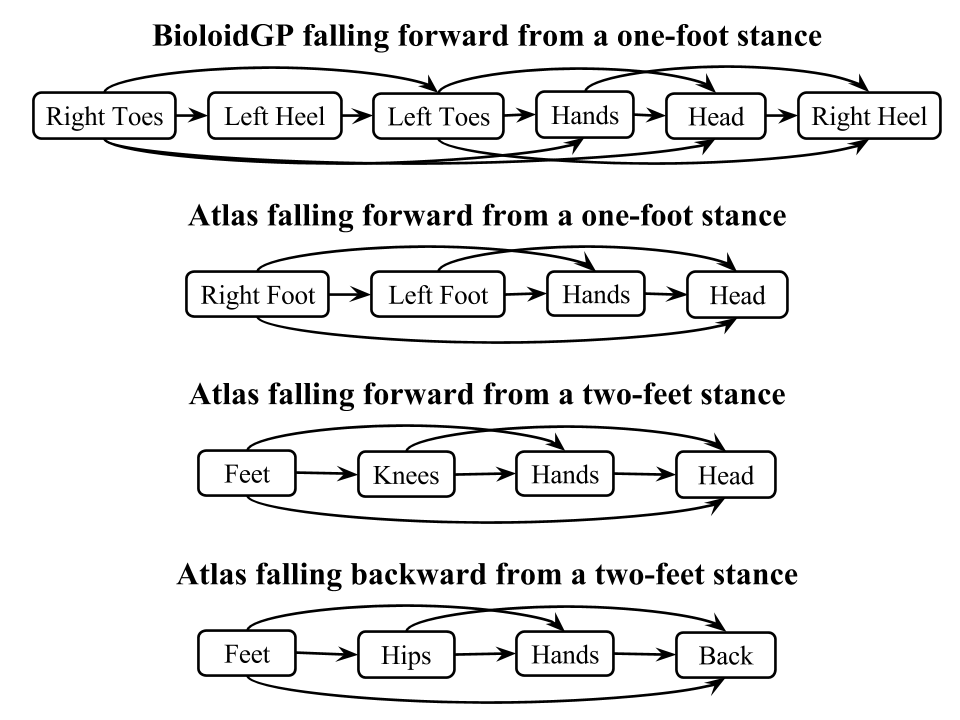
\includegraphics[width=3.2in]{images/all_contact_graphs.png}
%%   \caption{\updated{More contact graphcs are represented.
%%       Top: a forward fall of BioloidGP from one feet
%%       Middle: a forward fall of Atlas from one feet
%%       Bottom: a backward fall of Atlas from two feet}
%%     \sehoon{Will it be better to merge this with the previous contact graph
%%       figure (Figure. 2)?}}
%%   \label{fig:falling_all_contact_graphs}
%% \end{figure}

\begin{figure*}[ht]
\center
  %% 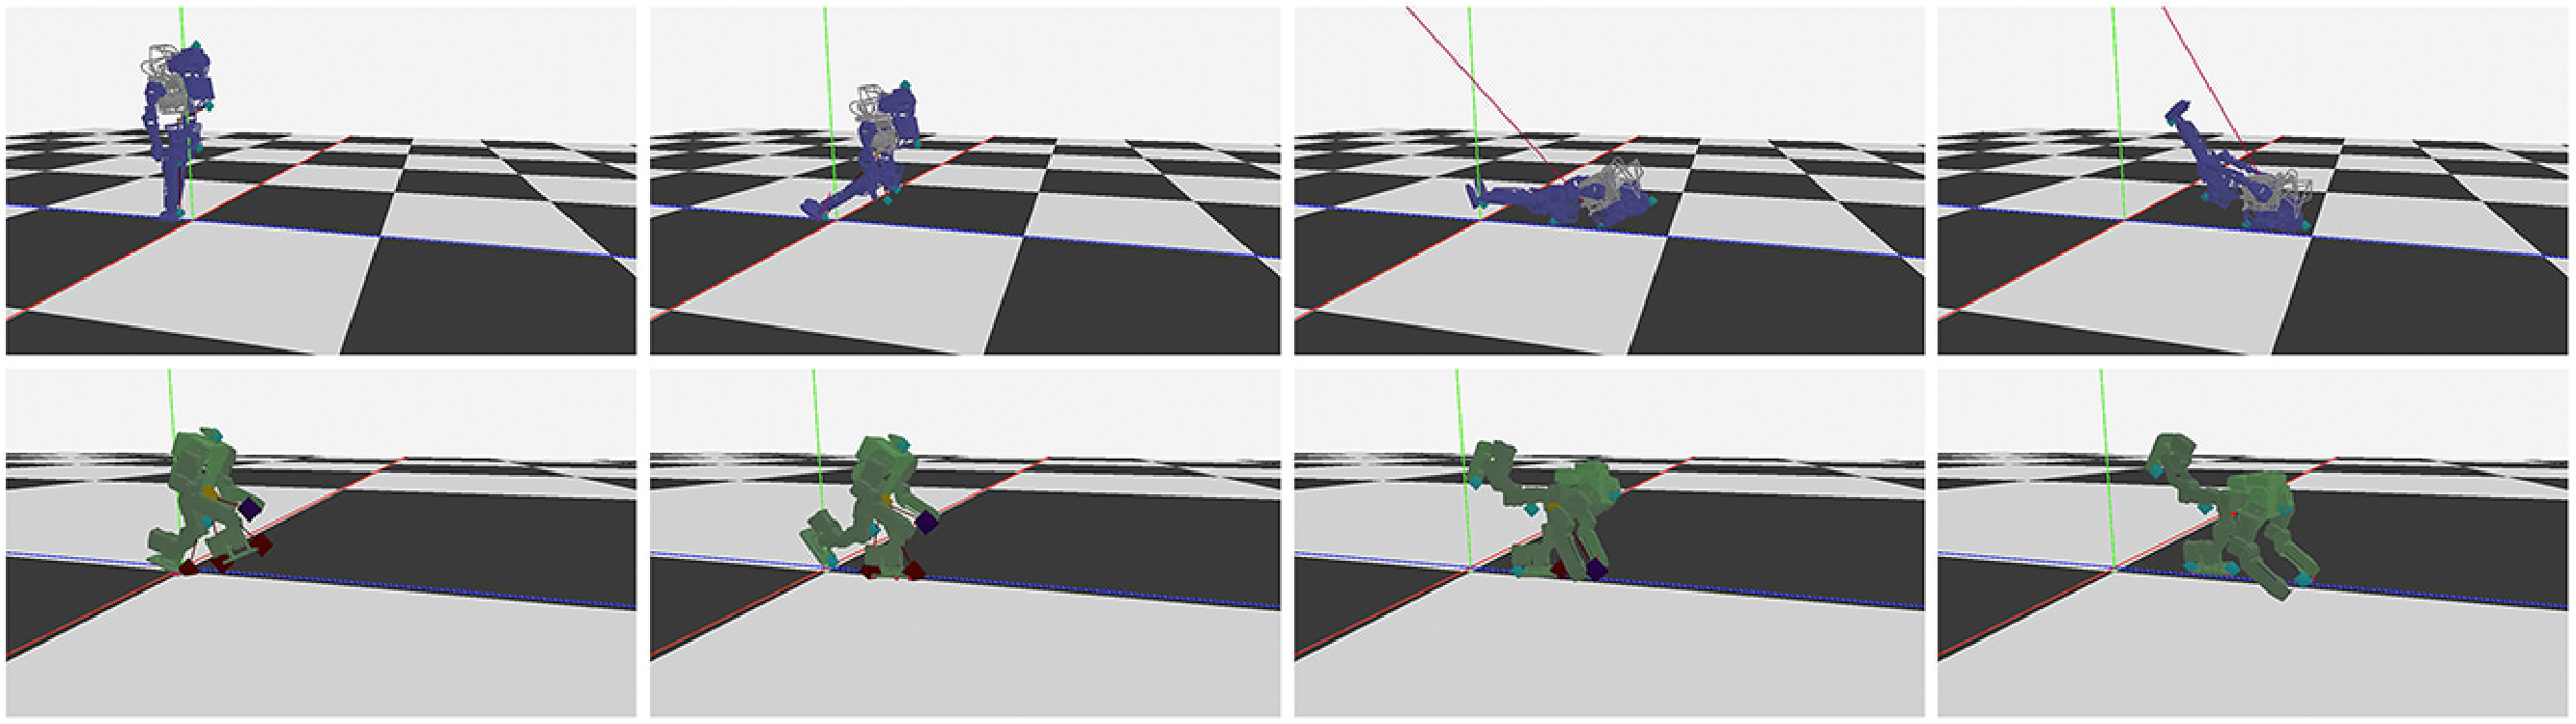
\includegraphics[width=6.8in]{images/falling_motions.pdf}
\setlength{\tabcolsep}{1pt}
\renewcommand{\arraystretch}{0.5}
\begin{tabular}{c c c c}
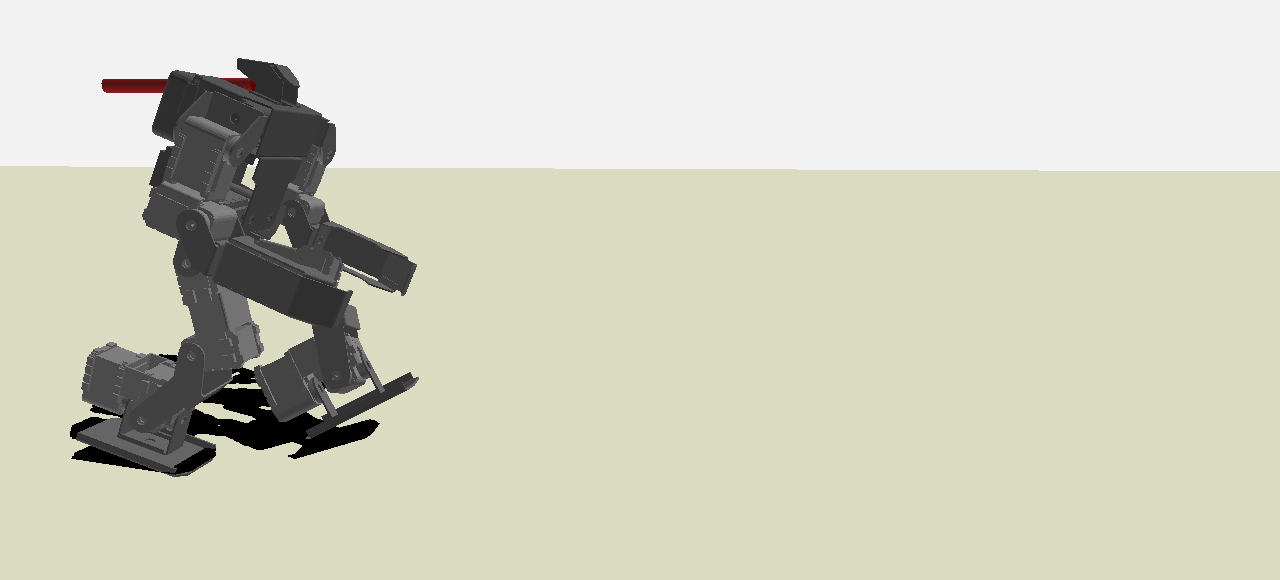
\includegraphics[width=0.24\textwidth]{images/GP_A_0.png}&
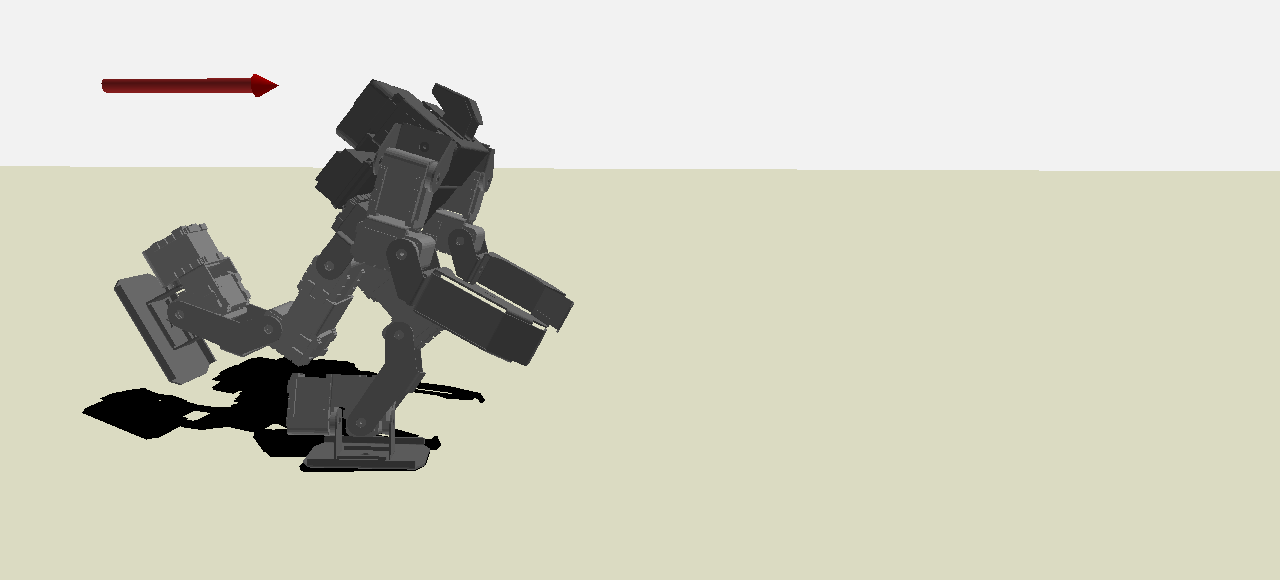
\includegraphics[width=0.24\textwidth]{images/GP_A_1.png}&
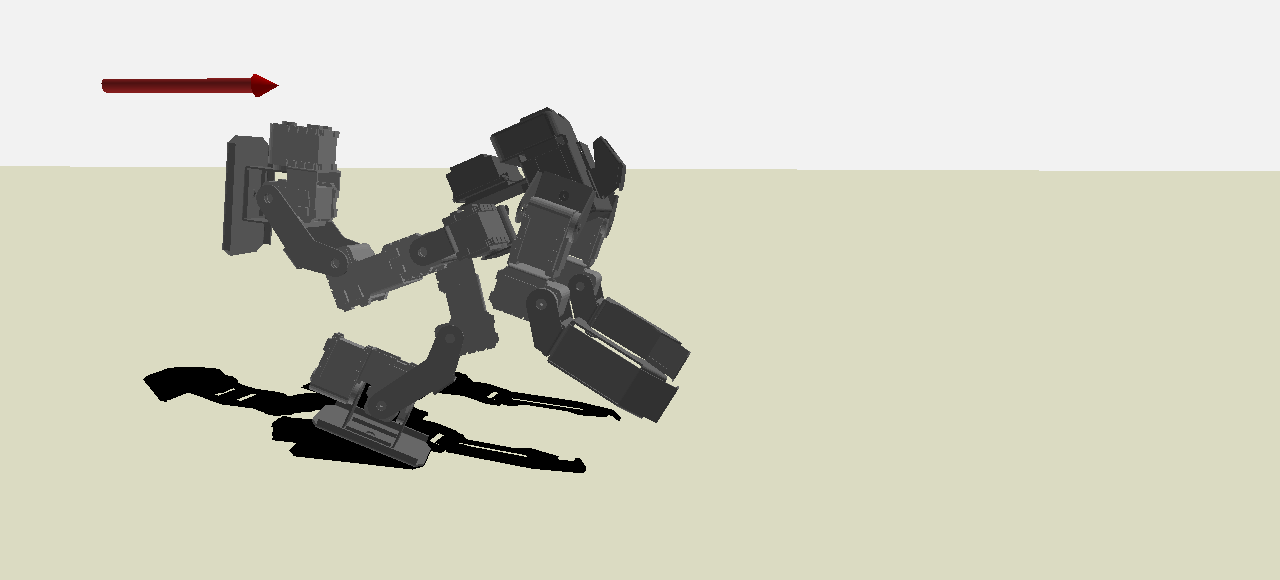
\includegraphics[width=0.24\textwidth]{images/GP_A_2.png}&
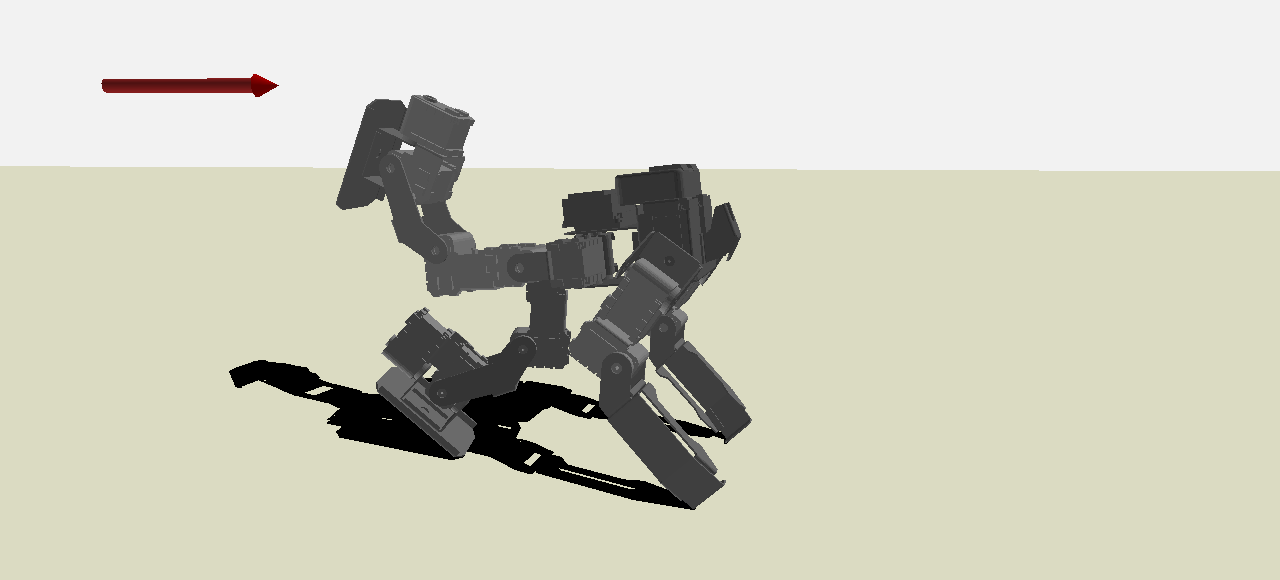
\includegraphics[width=0.24\textwidth]{images/GP_A_3.png} \\
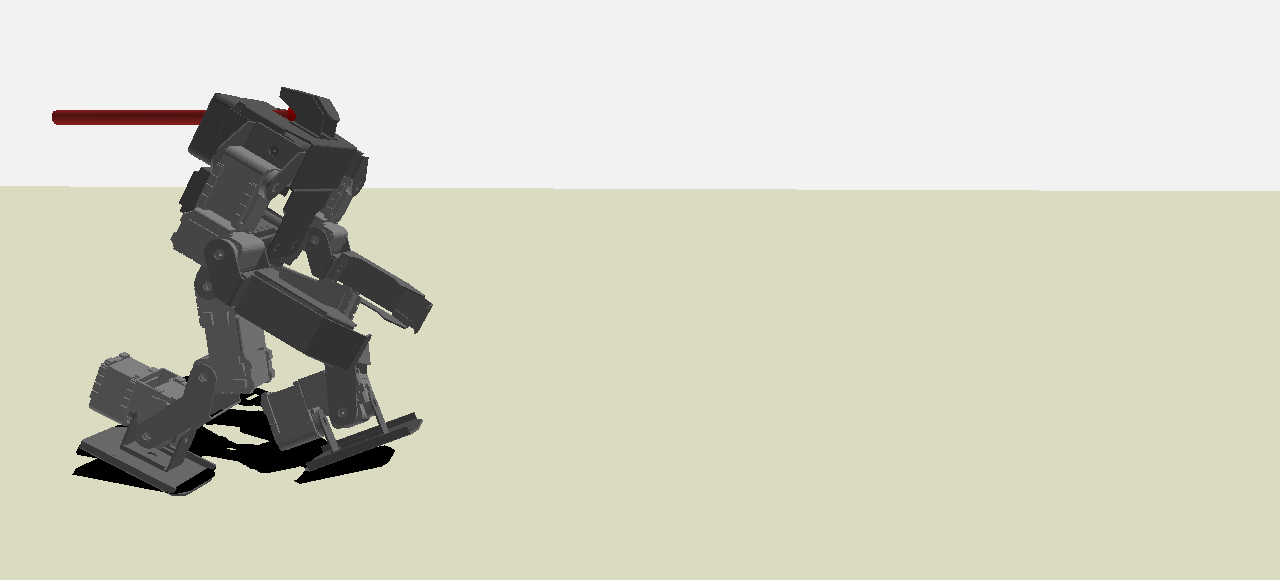
\includegraphics[width=0.24\textwidth]{images/GP_B_0.png}&
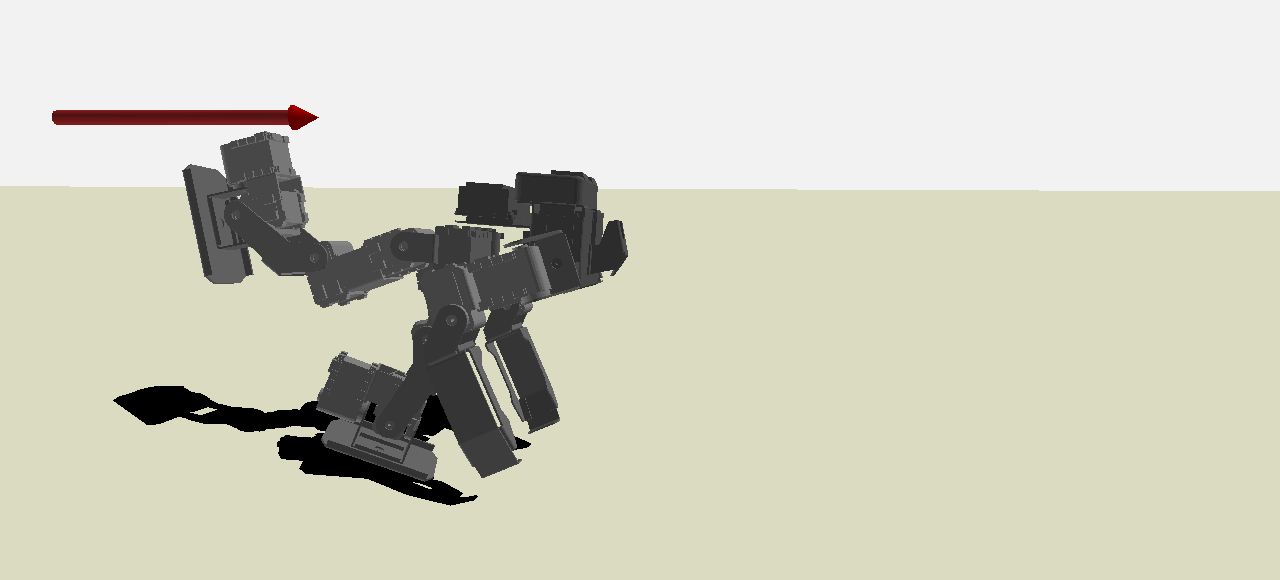
\includegraphics[width=0.24\textwidth]{images/GP_B_1.png}&
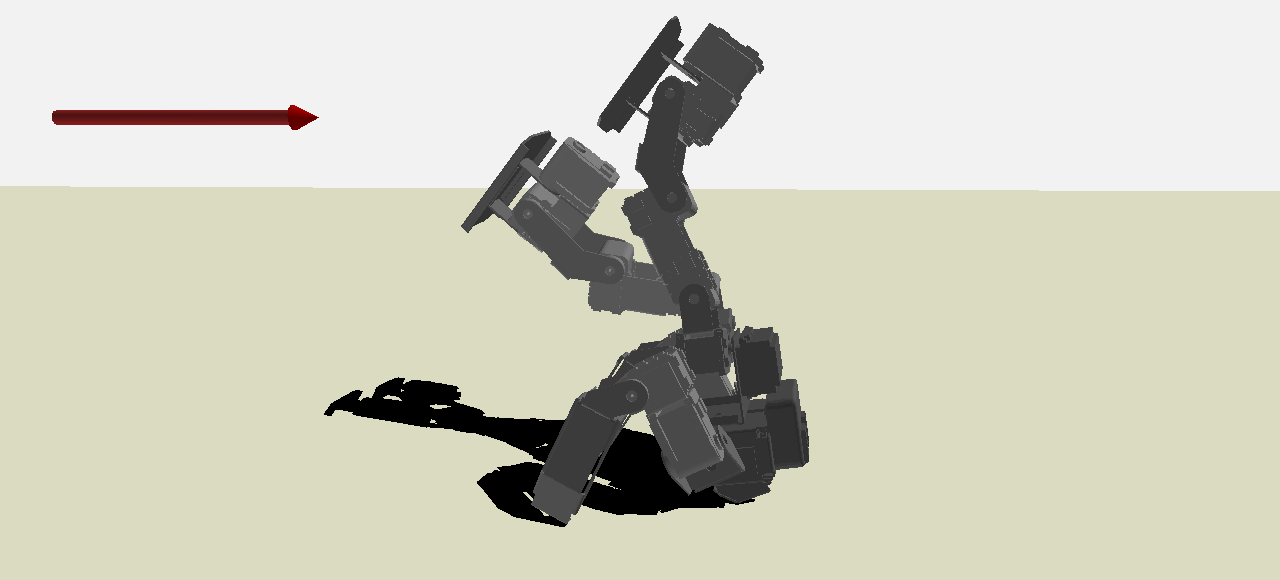
\includegraphics[width=0.24\textwidth]{images/GP_B_2.png}&
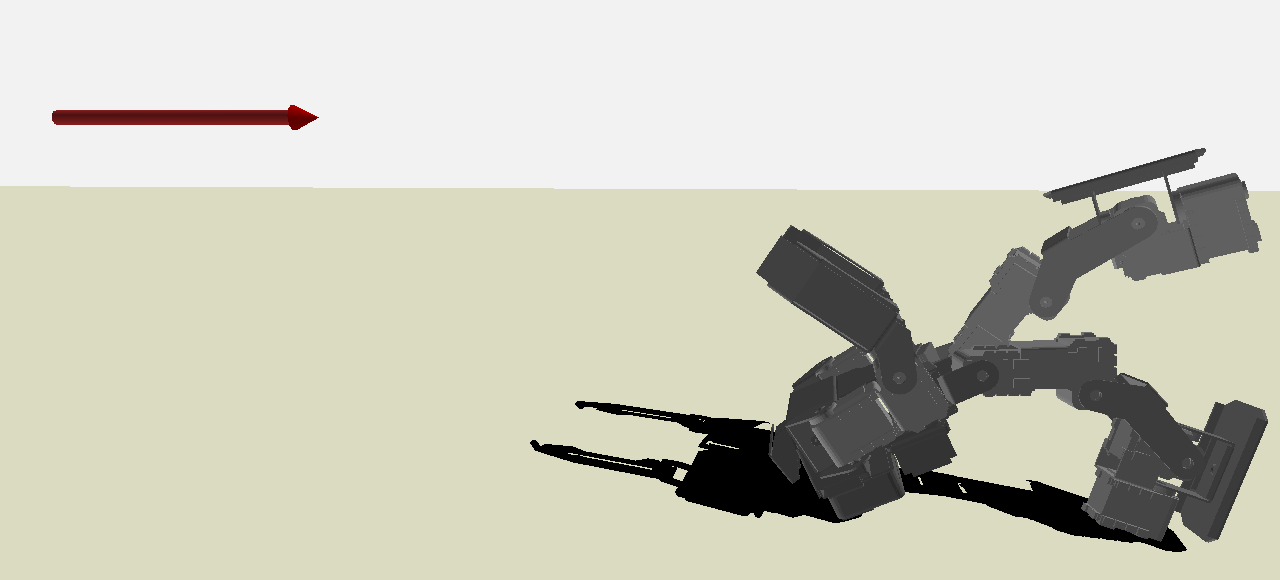
\includegraphics[width=0.24\textwidth]{images/GP_B_3.png} \\
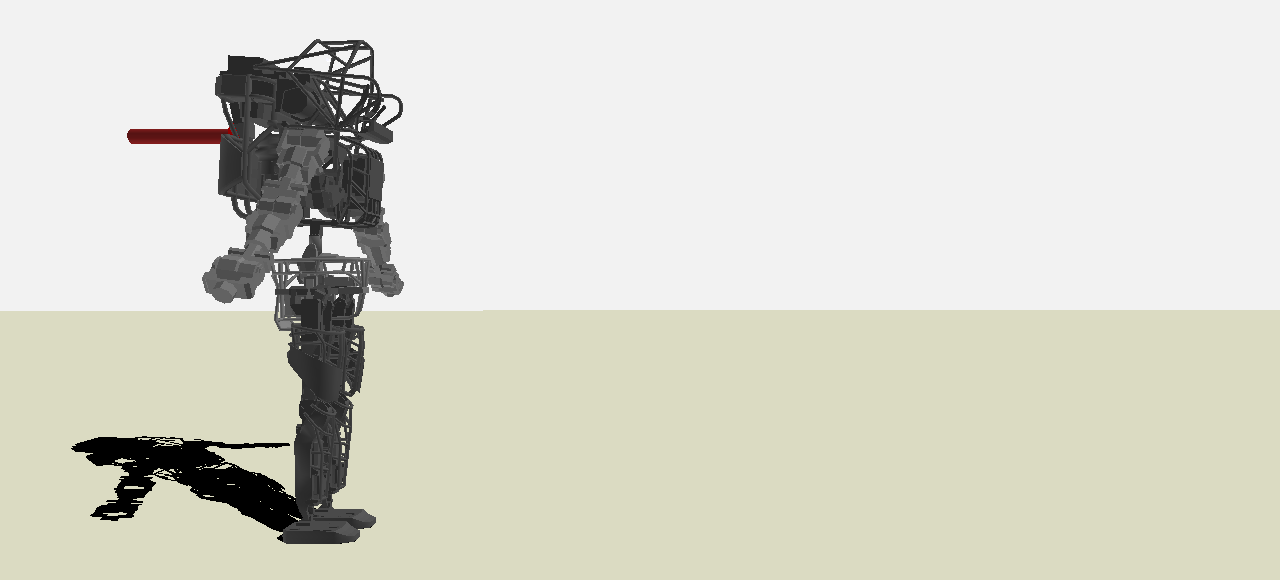
\includegraphics[width=0.24\textwidth]{images/Atlas_A_0.png}&
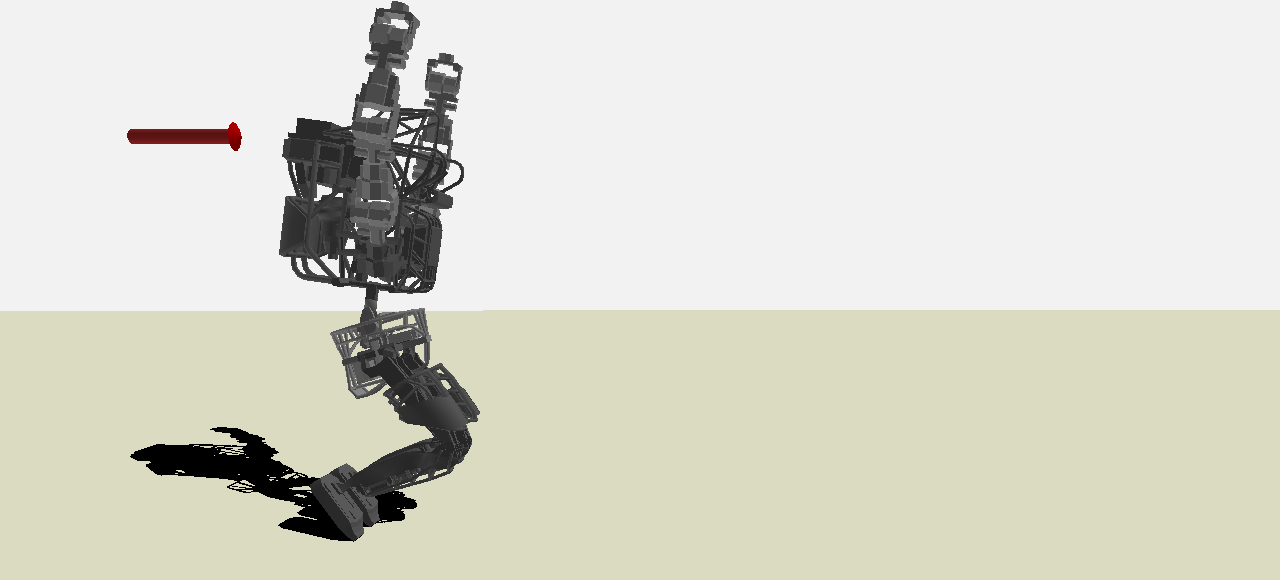
\includegraphics[width=0.24\textwidth]{images/Atlas_A_1.png}&
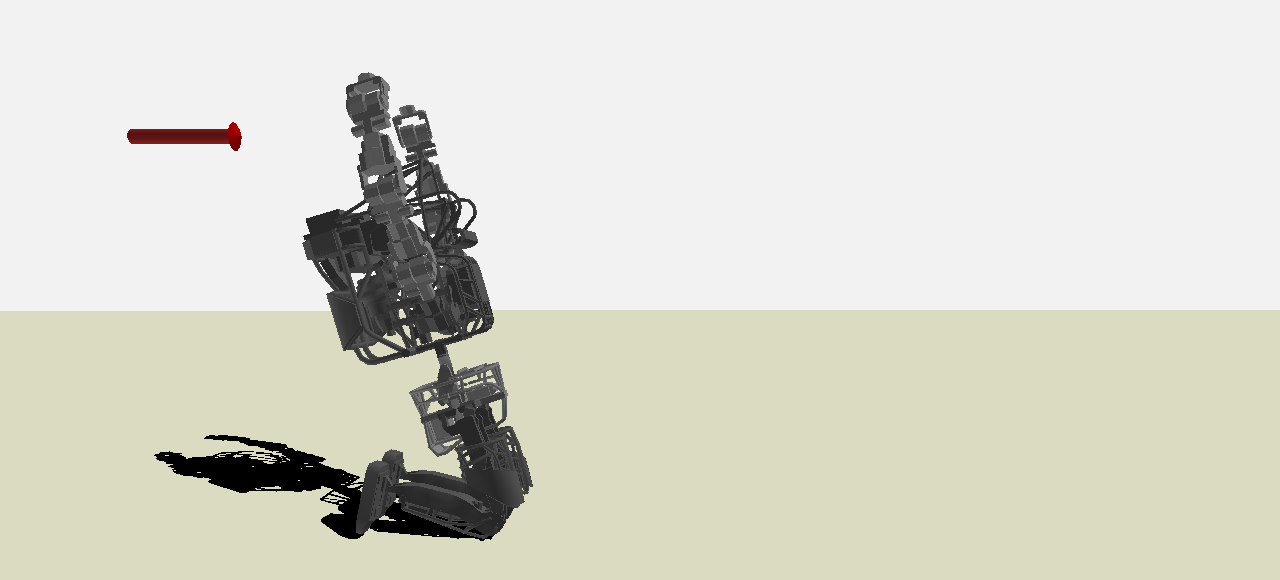
\includegraphics[width=0.24\textwidth]{images/Atlas_A_2.png}&
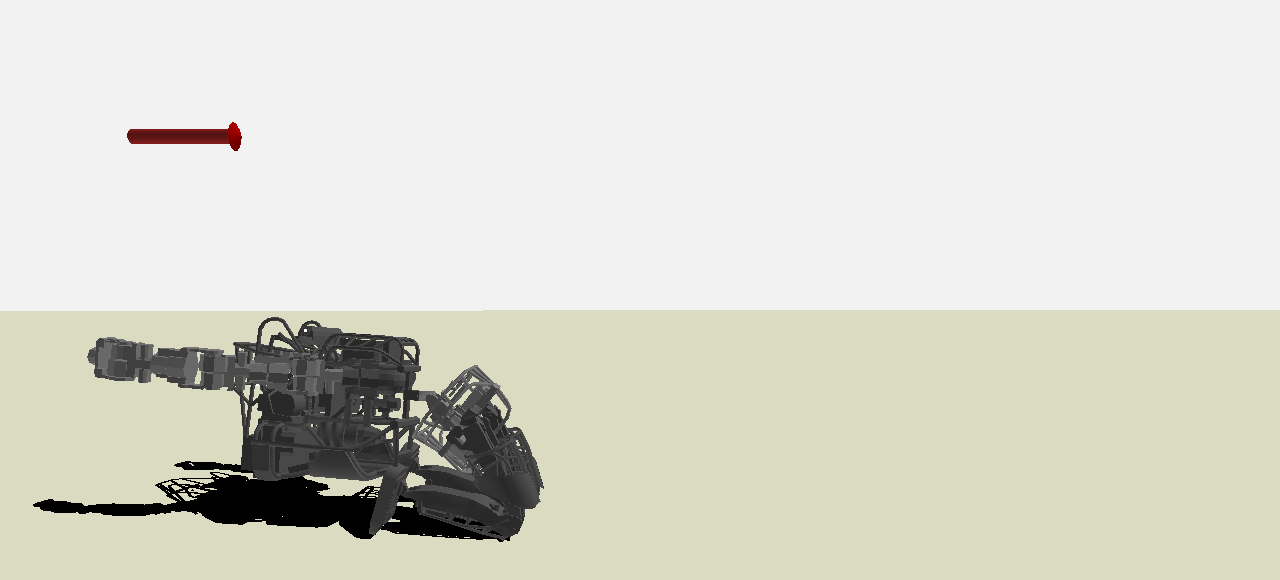
\includegraphics[width=0.24\textwidth]{images/Atlas_A_3.png} \\
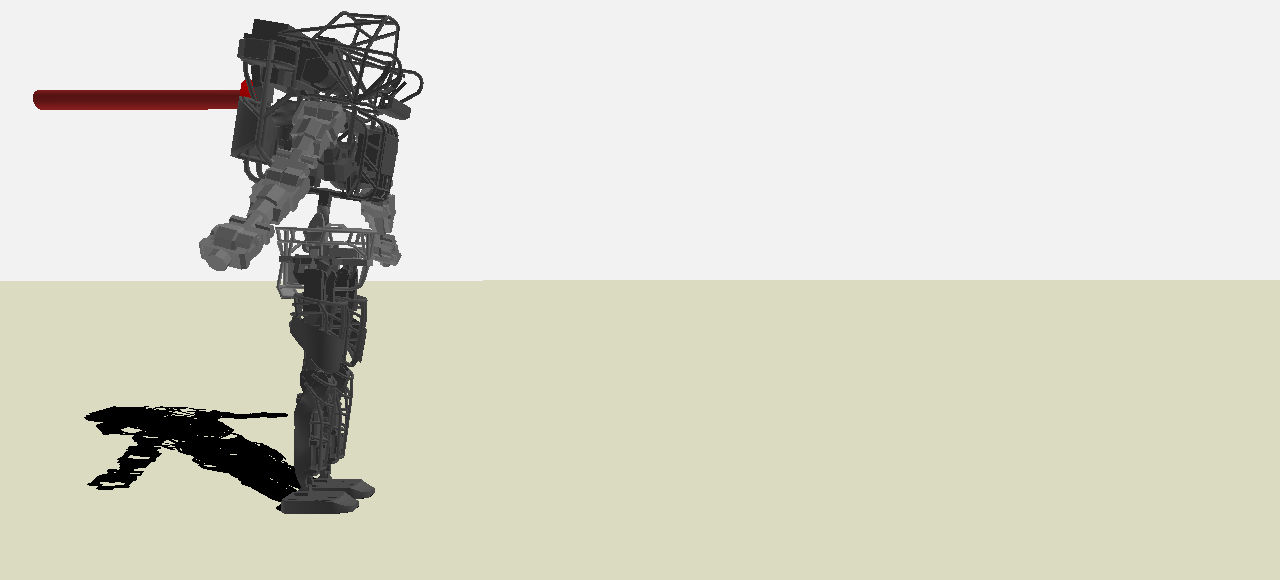
\includegraphics[width=0.24\textwidth]{images/Atlas_B_0.png}&
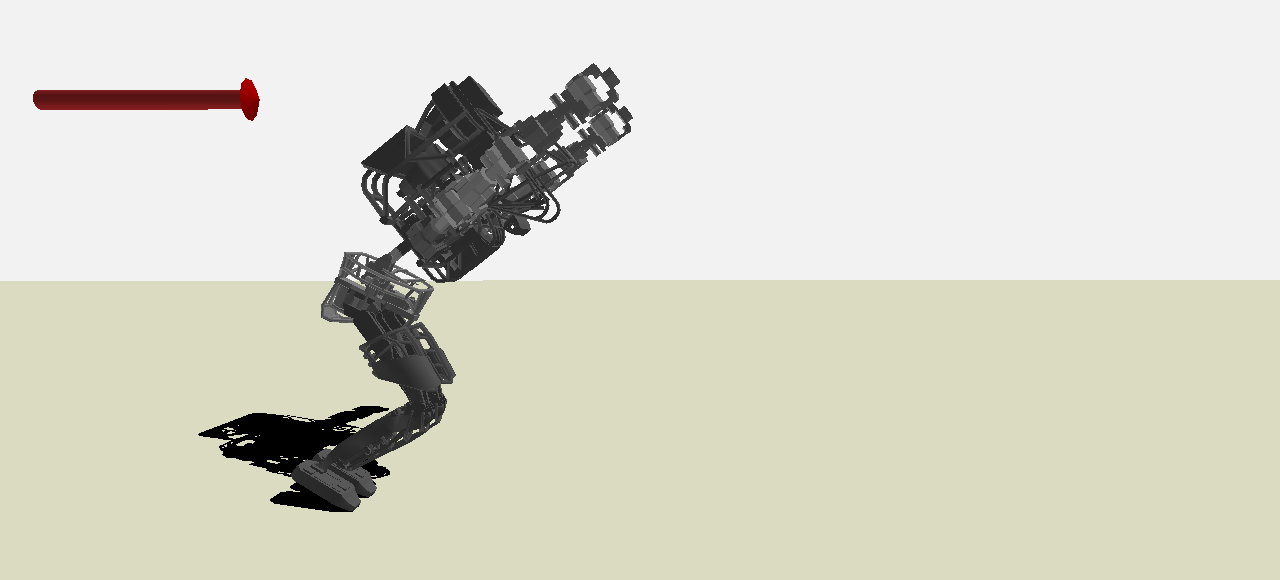
\includegraphics[width=0.24\textwidth]{images/Atlas_B_1.png}&
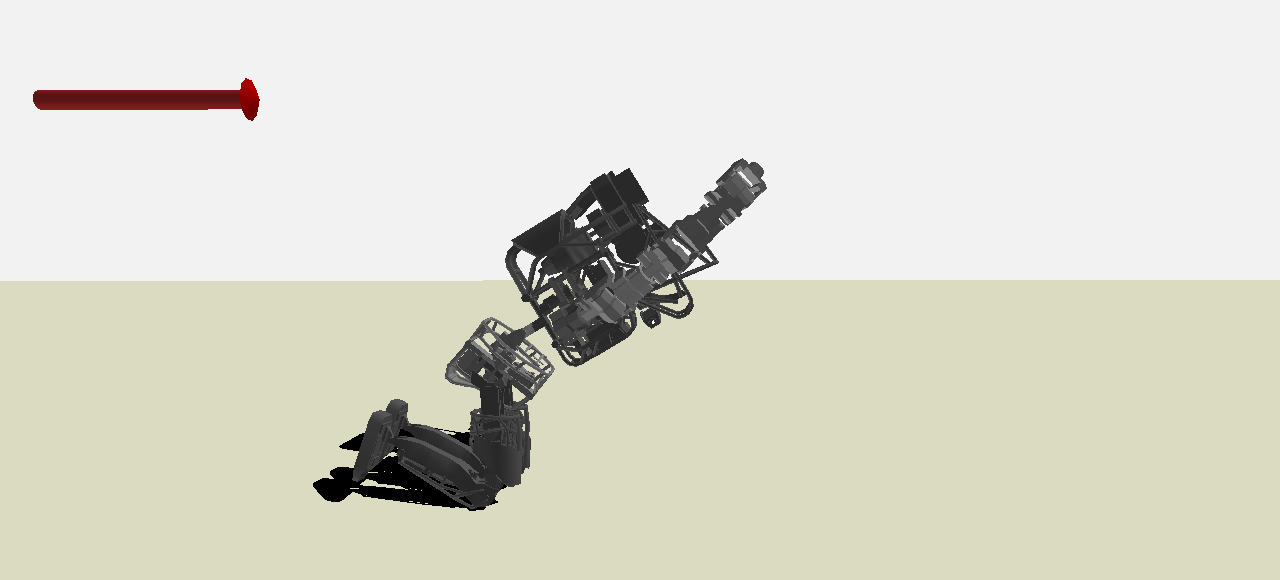
\includegraphics[width=0.24\textwidth]{images/Atlas_B_2.png}&
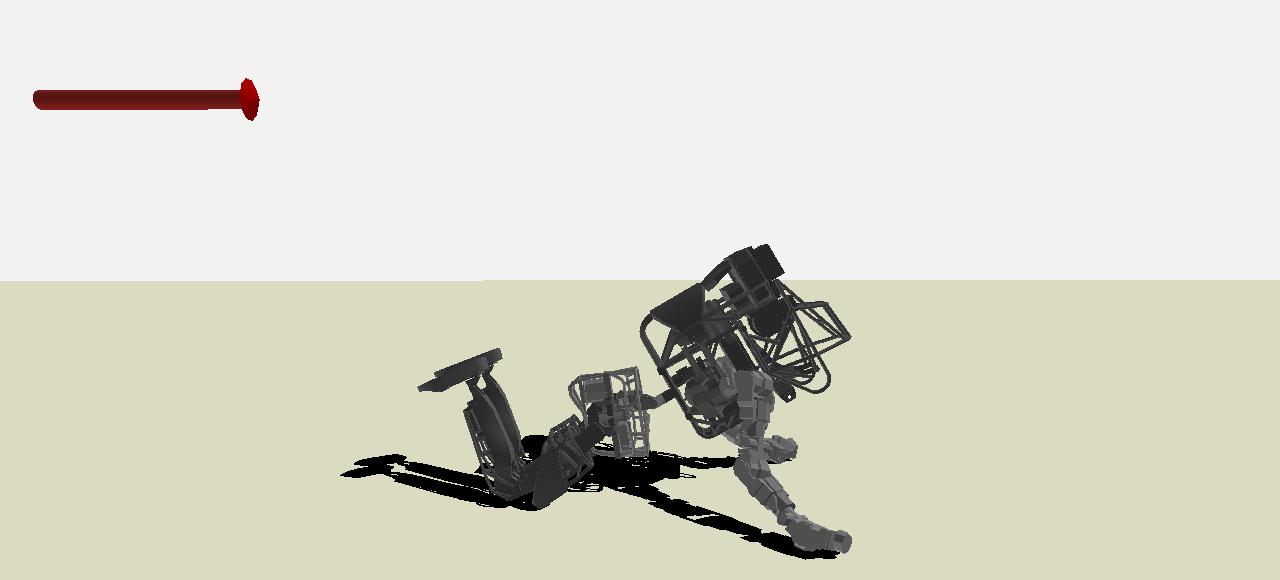
\includegraphics[width=0.24\textwidth]{images/Atlas_B_3.png} \\
\end{tabular}
\caption{First row: BioloidGP forward falling from a one-foot
    stance due to a $5.0$N push. Second row: BioloidGP forward falling
    from a one-foot stance due to a $8.0$N push. Third row: Atlas
    forward falling from a two-feet stance due to a $1000$N push. Fourth
    row: Atlas forward falling from a two-feet stance due to a
    $2000$N push.}
  \label{fig:falling_motions}
\end{figure*}

%%%%%%%%%%%%%%%%%%%%%%%%%%%%%%%%%%%%%%%%%%%%%%%%%%%%%%%%%%%%%%%%%%%%%%%%%%%%%%%%
\subsubsection{BioloidGP}
BioloidGP is a small humanoid robot with $16$ degrees of freedom (DOFs)
($34.6$cm, $1.6$kg). Our first set of tests applied pushes with
different magnitudes to the robot. Starting with the same one-foot
stance, we ran four tests with pushes ranging from $0.5$N to $8.0$N,
applied for $0.1$ second at beginning of the fall. We set the joint
angle limits at $\pm150^{\circ}$ and the torque limits at $0.6Nm$. We
approximated the speed limit of the COM in the vertical direction and
set the limits of the rod length velocity $\dot{r}_1^d$ at
$\pm0.03m/s$. The input contact graph is shown in
\figref{falling_contact_graph}.  Due to the relatively large feet of
BioloidGP, heels and toes were treated as two separate contacts.

%% \sehoon{How about denote ``\# of contacts'' in \tabref{falling_gp_results}
%%   instead of the full sequence of contacts? In that case, we can make
%%   the table as one column. We can explain the sequence in the text and
%%   video.}
%% \karen{I like the entire contact sequence in the table, unless we need
%%   to save space.}

%%%%%%%%%%%%%%%%%%%%%%%%%%%%%%%%%%%%%%%%
% Table begins
\begin{table*}
\scriptsize
\center
{
\caption{The initial conditions and the results of BioloidGP simulations.
}
\begin{tabular}{c |c c c|l | l}
\label{tab:falling_gp_results}
\\ \hline
Mag.(N) & Unplanned & Planned & Ratio & Contacts & Remarks \\ \hline
0.5 & 0.8889 & 0.2063 & 23.2\% & right toes, left heel, left toes & Stepping\\ \hline
1.5 & 0.6789 & 0.2776 & 40.9\% & right toes, left heel, left toes, hands & Tripod\\ \hline
5.0 & 0.9312 & 0.3885 & 41.7\% & right toes, left heel, left toes, hands & Tripod \\ \hline
8.0 & 1.2170 & 0.5884 & 48.4\% & right toes, left heel, left toes, hands, head, right heel & Rolling \\ \hline
\end{tabular}
}
\end{table*}
%%%%%%%%%%%%%%%%%%%%%%%%%%%%%%%%%%%%%%%%
\tabref{falling_gp_results} describes the details of the initial conditions
and the results of each test. The columns of the table denote the
magnitude of perturbation, the maximum impulses of the unplanned and
the planned motions, the impact ratio of planned to unplanned motion,
the optimal contact sequence, and a short description of the
emergent falling strategy. As we expected, our planning algorithm used more
contacts when the initial momentum was large. For a push with $0.5$N,
the robot took a single step to recover the fall. For the cases of
$1.5$N and $5.0$N, our algorithm planned a contact sequence with the
left heel, the left toe, and both hands, reminiscent to the Tripod strategy
proposed by \cite{Yun:2014:TFC}. When we increased the magnitude of the
push to $8.0$N, the rolling strategy, effective for breaking high
speed falls \cite{ZenpoUkemi:2014:URL}, automatically emerged. Please
refer to the supplementary video and \figref{falling_motions} for all the
results.

\begin{figure}[ht]
\center
  %% 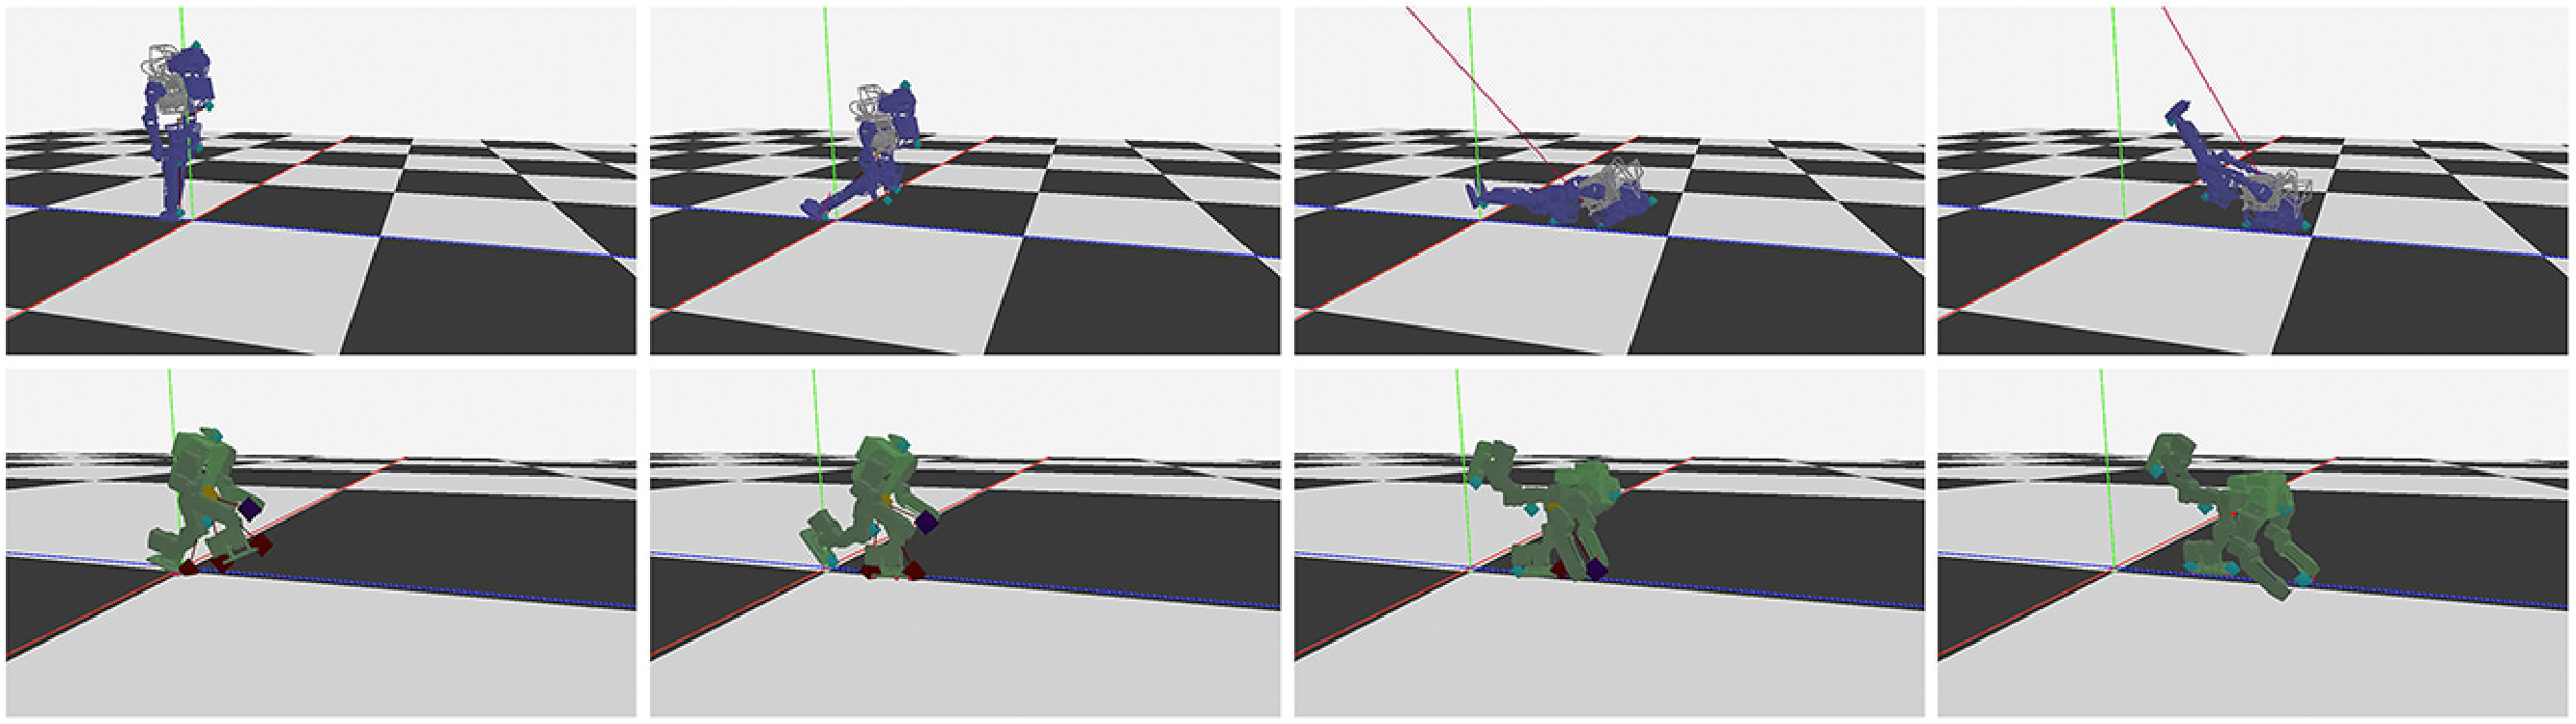
\includegraphics[width=6.8in]{images/falling_motions.pdf}
\setlength{\tabcolsep}{1pt}
\renewcommand{\arraystretch}{0.5}
\begin{tabular}{c c}
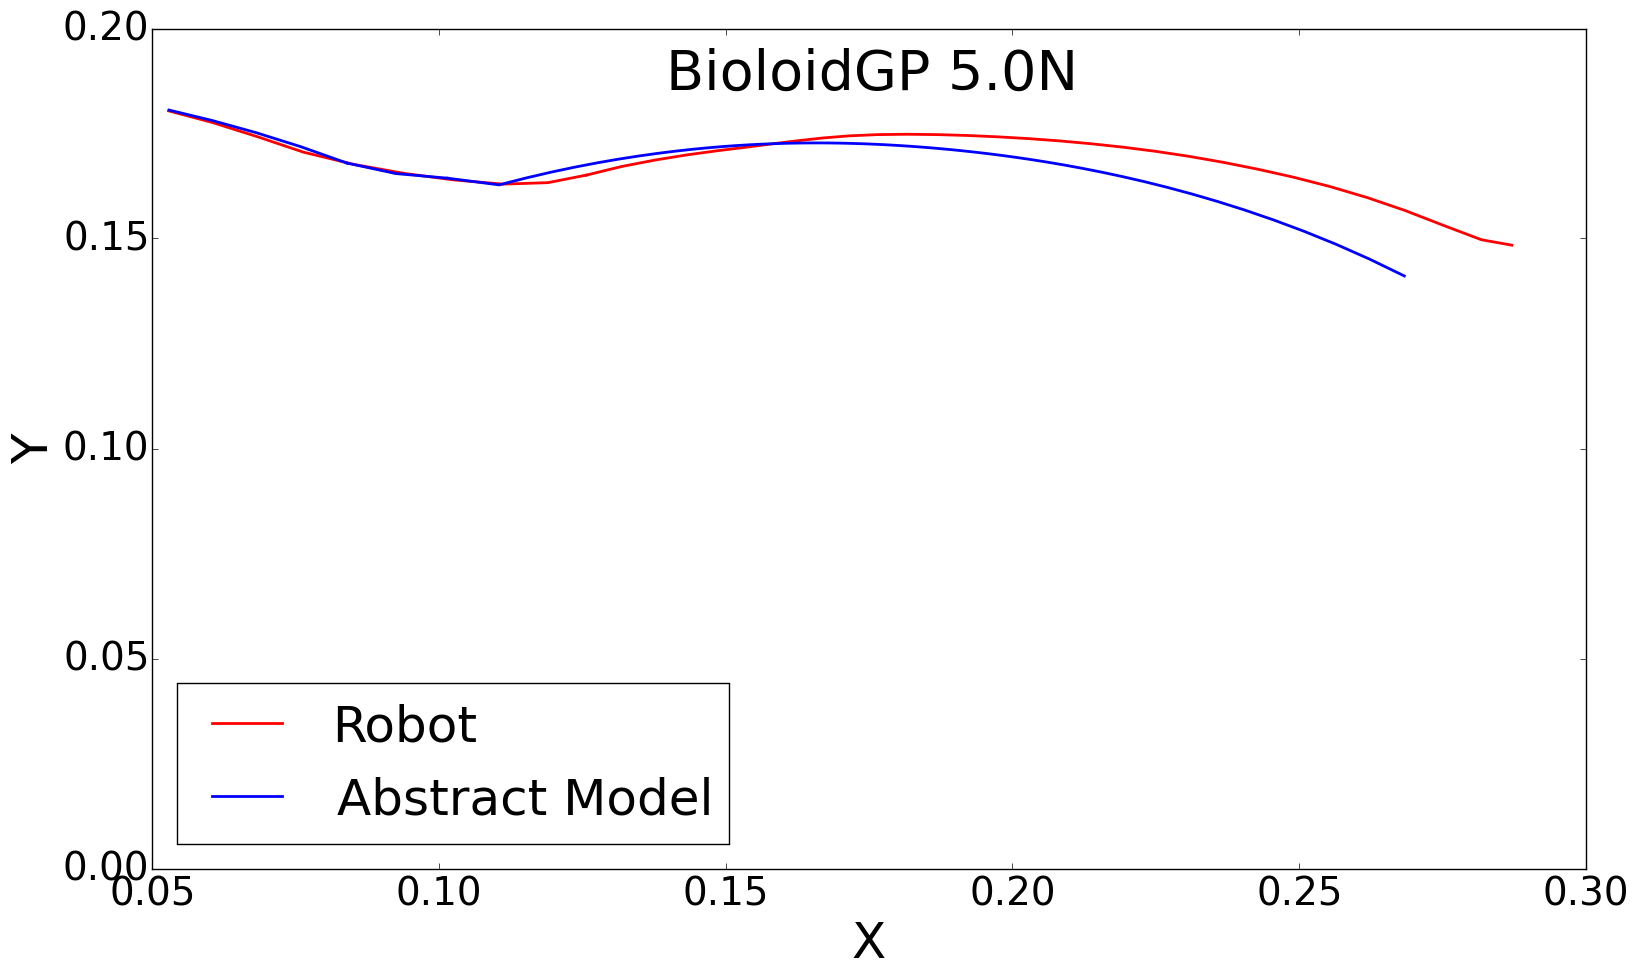
\includegraphics[width=2.2in]{images/COM_GP_A.png}&
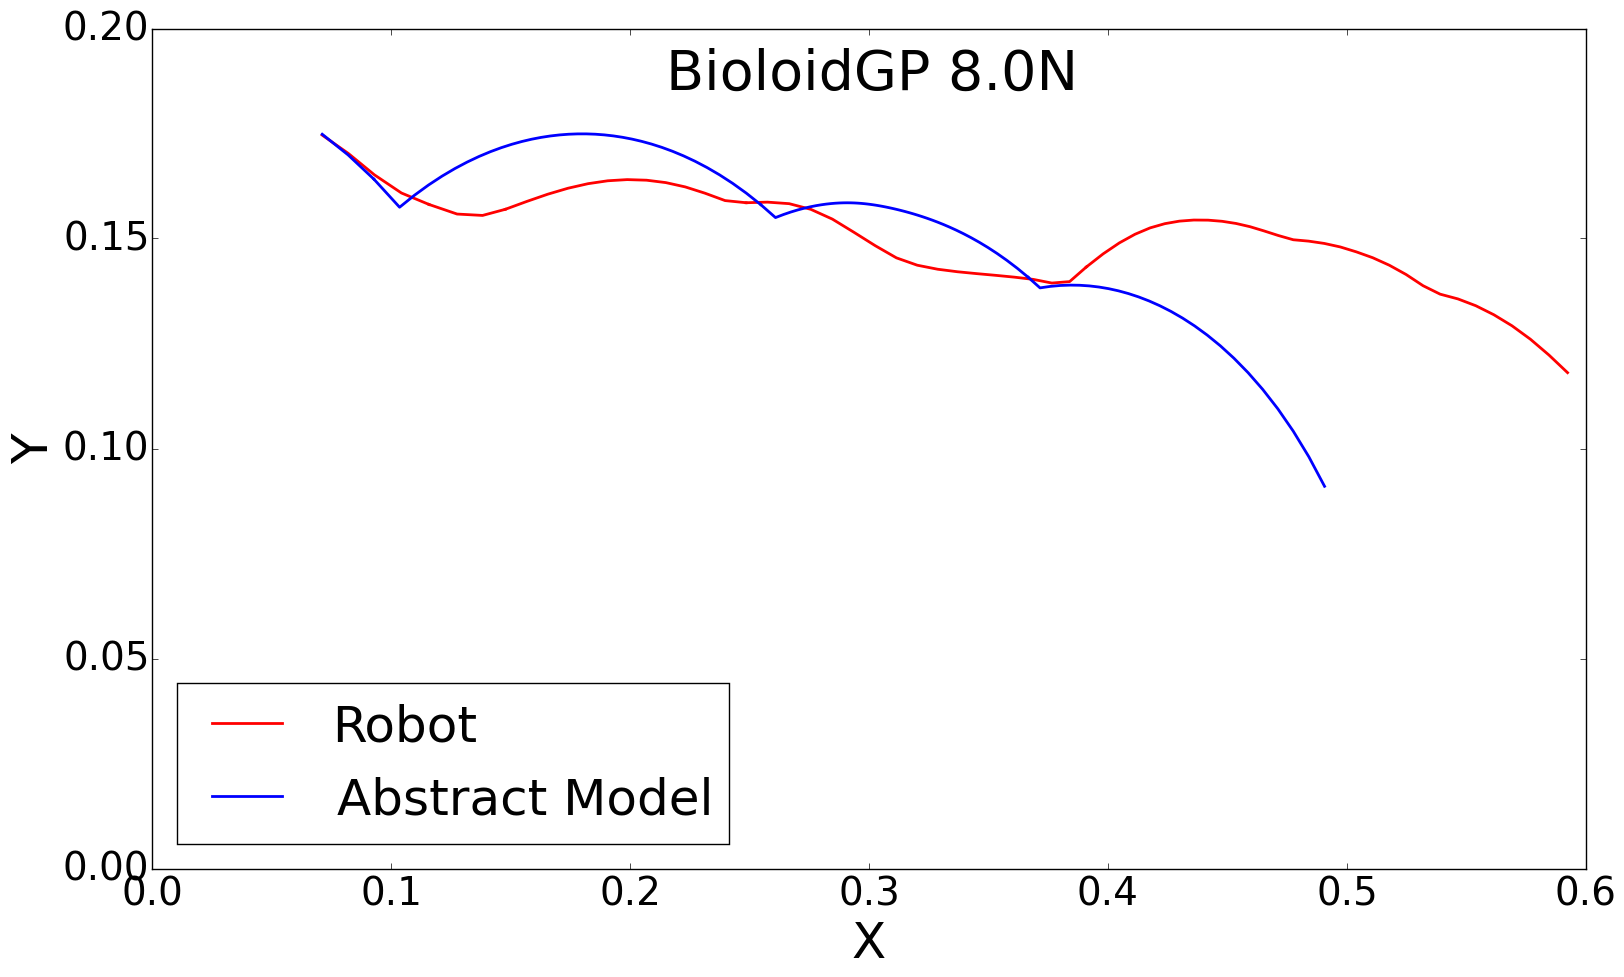
\includegraphics[width=2.2in]{images/COM_GP_B.png}\\
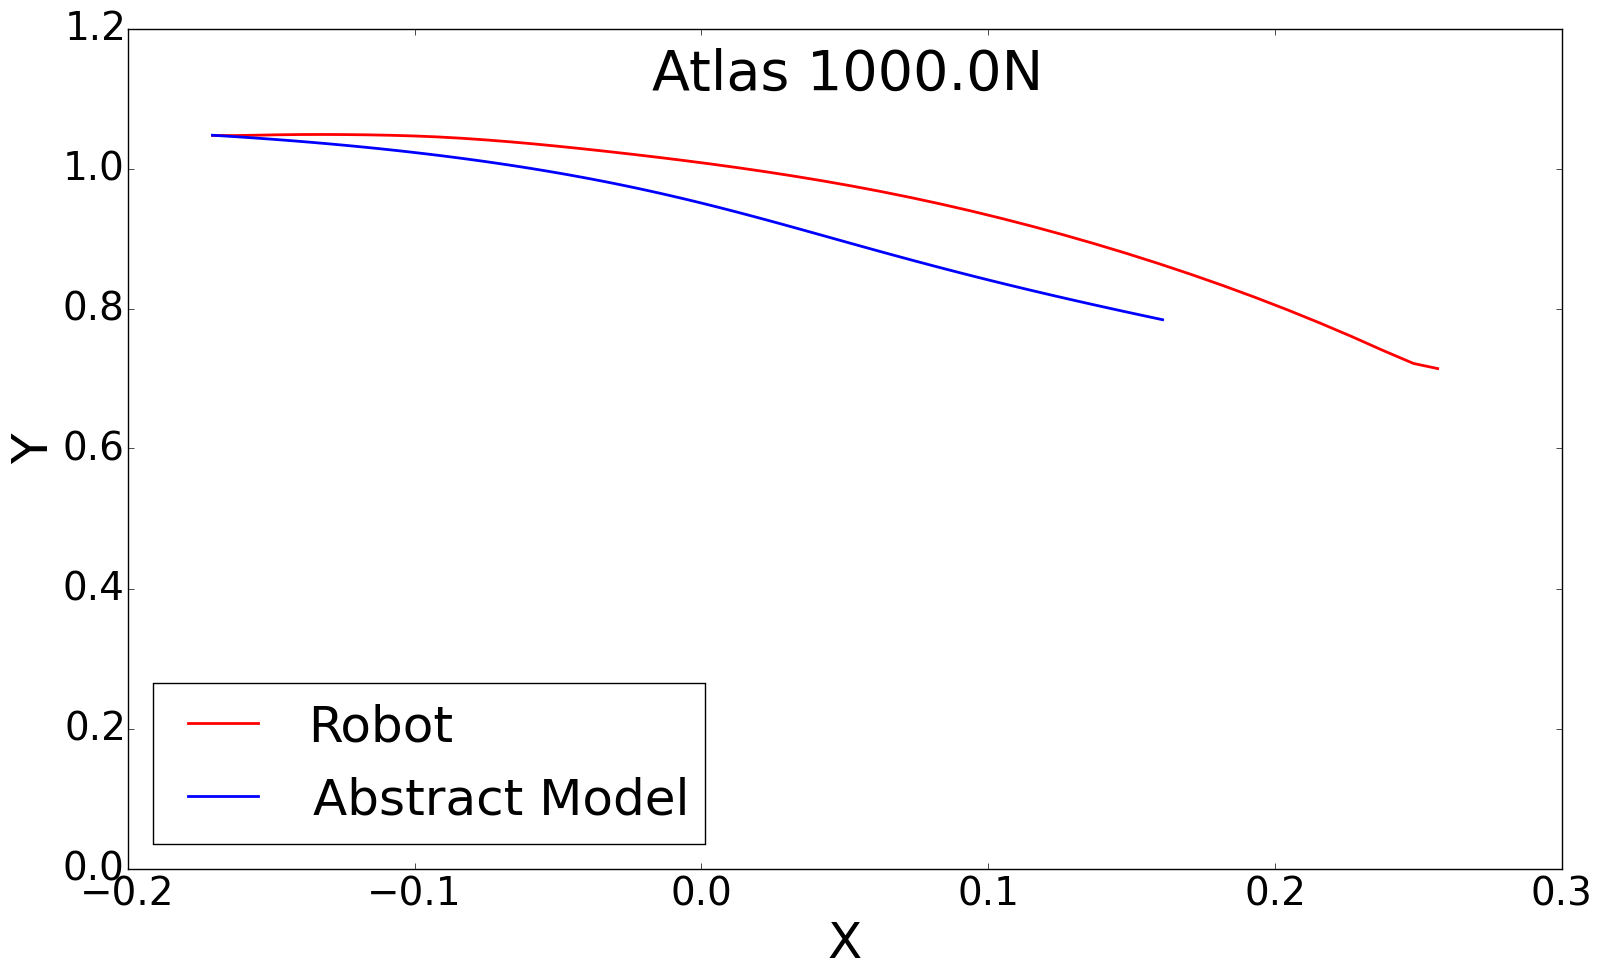
\includegraphics[width=2.2in]{images/COM_Atlas_A.png}&
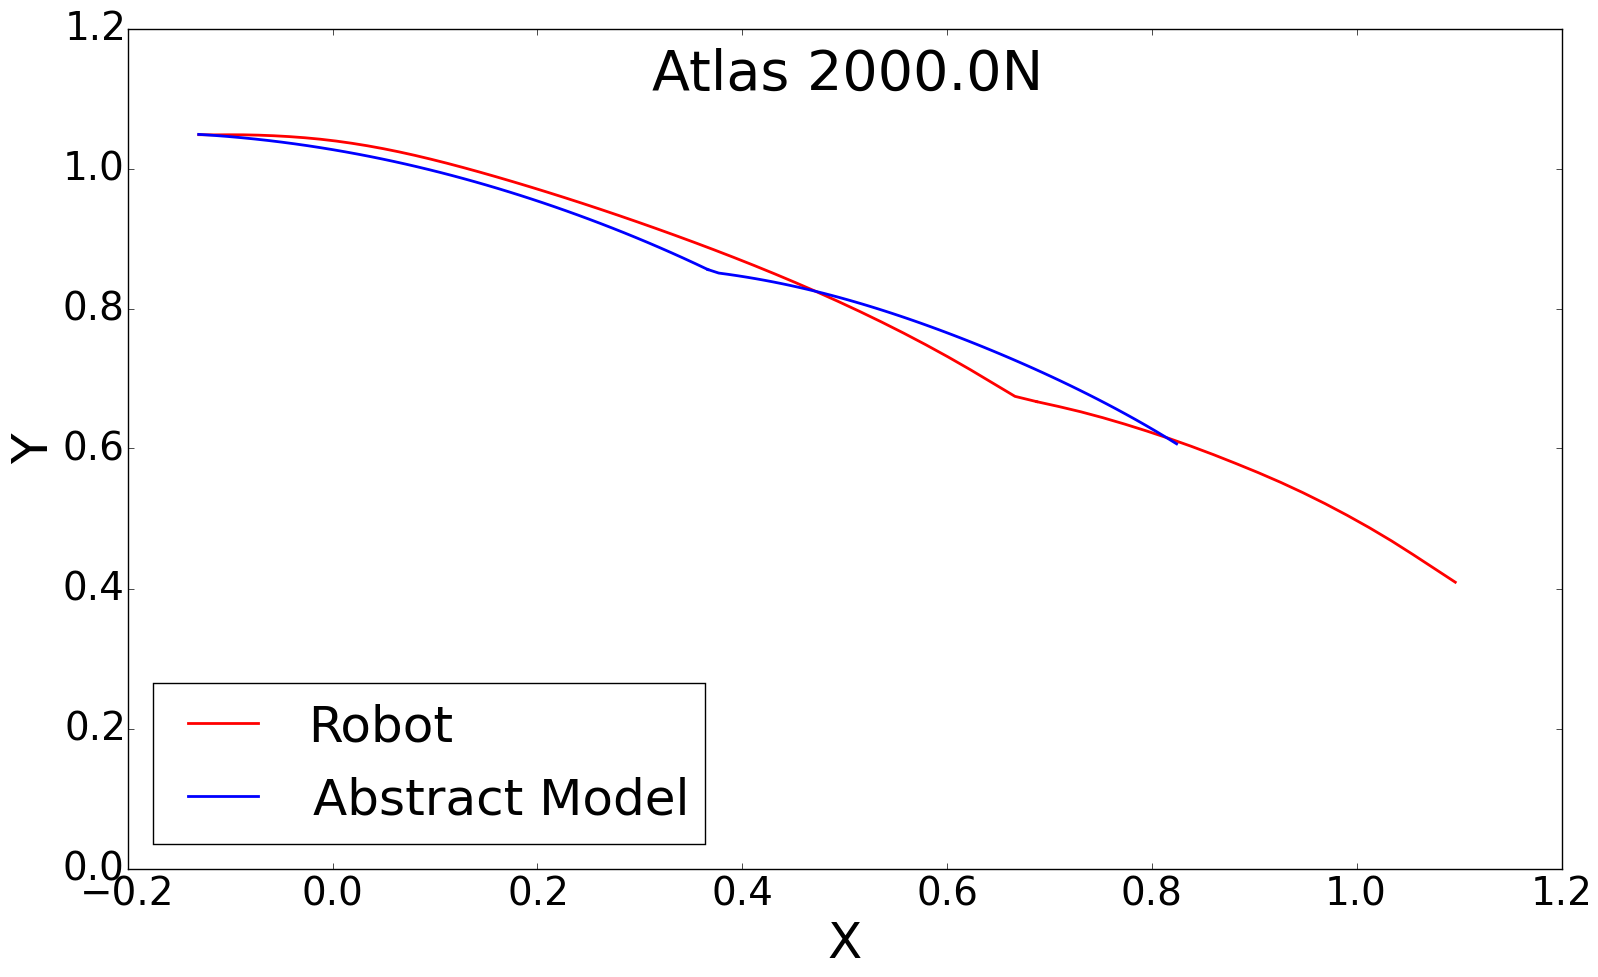
\includegraphics[width=2.2in]{images/COM_Atlas_B.png}\\
\end{tabular}

  \caption{COM trajectories between the abstract model
      (Blue) and the robot (Red). 
      Top left: BioloidGP forward falling from a one-foot stance due to a
      $5.0$N push. Top right: BioloidGP forward falling from a one-foot stance
      due to a $8.0$N push. Bottom left: Atlas forward falling from a two-feet
      stance due to a $1000$N push. Bottom right: Atlas forward falling 
      from a two-feet stance due to a $2000$N push.}
  \label{fig:falling_coms}
\end{figure}

Comparing to unplanned motions, our algorithm only caused $23.2\%$ to
$48.4\%$ of the maximum impulse. To verify how well the
contact plan $\mathcal{P}$ was executed, we compared the COM
trajectories between the abstract model and the robot
(\figref{falling_coms}). Most plans were executed well with an exception of the
$8.0$N case due to the accumulated errors over a longer motion
sequence. Still, in this case the maximum impulse was significantly
reduced due to the distribution of impulse over multiple contacts.

The contact graph is an important input that defines all possible
contact sequences for the given humanoid. We ran an additional test to
modify the contact graph of the BioloidGP robot. By removing the
``hands'' node, the $8.0$N push resulted in a hands-free rolling sequence.
  % The maximum impulse of the new motion is $0.9890$Ns that is between the
  % original strategy ($0.5884$Ns) and the unplanned motion ($1.2170$Ns).}
  %% However, it results the higher maximum impulse ($0.9890$Ns) than the original
  %% strategy ($0.5884$Ns) that is still lower than the unplanned motion
  %% ($1.2170$Ns). }

%%%%%%%%%%%%%%%%%%%%%%%%%%%%%%%%%%%%%%%%%%%%%%%%%%%%%%%%%%%%%%%%%%%%%%%%%%%%%%%%
\subsubsection{Atlas}
We also evaluated our algorithm on a large humanoid, Atlas ($188$cm,
$150$kg, $28$DOFs).  We followed the joint limits and the torque
limits described in the URDF file provided by Boston Dynamics
\cite{BD:2014:URL}. The limits of the rod length velocity
$\dot{r}_1^d$ were set at $\pm0.3m/s$.  We ran six test cases with
three initial settings: a forward push from a one-foot stance pose, a
forward push from a two-feet stance pose, and a backward push from a
two-feet stance pose. For each setting, we pushed the robot with two
different magnitudes.  The input contact graphs are shown in
\figref{falling_contact_graph}.

%%%%%%%%%%%%%%%%%%%%%%%%%%%%%%%%%%%%%%%%
% Table begins
\begin{table*}
\scriptsize
\center
{
\caption{The initial conditions and the results of Atlas simulations.}
\begin{tabular}{c c c|c c c| l }
\label{tab:falling_atlas_results}
\\ \hline 
Initial Stance & Direction & Mag.(N) & Unplanned(Ns) & Planned(Ns) & Ratio & Contacts \\ \hline
One foot & Forward & 1000 & 363.9 & 37.8 & 10.4\% & right foot,  left foot \\ \hline
One foot & Forward & 2500 & 401.5 & 281.1 & 70.0\% & right foot,  left foot, hands \\ \hline
Two feet & Forward & 1000 & 392.8 & 214.0 & 54.5\% & feet, knees \\ \hline
Two feet & Forward & 2000 & 322.7 & 199.7 & 61.8\% & feet, knees, hands \\ \hline
Two feet & Backward & 300 & 338.8 & 176.5 & 52.1\% & feet, hands \\ \hline
Two feet & Backward & 500 & 344.6 & 243.9 & 70.8\% & feet, hips, hands, back \\ \hline
\end{tabular}
}
\end{table*}

\tabref{falling_atlas_results} shows the initial settings and the results for all
the tests. Again, our algorithm suggested to use more contacts for
pushes with higher magnitudes. For the same setting (falling forward
from a one-foot stance pose), we observed a change of strategy from taking a
small step ($1000N$) to using Tripod strategy ($2500N$).  In the case
of falling forward from a two-feet stance pose, the robot landed on its knees
when the push was weak ($1000N$), similar to the strategy proposed by
\cite{Fujiwara:2004:SKL}.  When the external force became stronger
($2000N$), the robot utilized an additional contact with hands,
similar to the strategy reported in
\cite{Fujiwara:2007:OPF,Ogata:2008:RSG}. For backward falls, the robot
was able to stop a gentle nudge ($300N$) using only hands but needed
to use three contacts, hips, hands, and back, to stop a stronger push
($500N$), similar to \cite{Fujiwara:2002:UFM}.  Please refer to the
supplementary video and \figref{falling_motions} for all the results.

Comparing to unplanned motions, our algorithm caused $10.4\%$ to
$70.8\%$ of the maximum impulse. Because Atlas has relatively short
arms, the backward falls presented more challenges than the forward
falls. The planned and executed COM trajectories for falling forward
from a two-feet stance pose are compared in \figref{falling_coms}.

%%%%%%%%%%%%%%%%%%%%%%%%%%%%%%%%%%%%%%%%%%%%%%%%%%%%%%%%%%%%%%%%%%%%%%%%%%%%%%%%
\subsection{Hardware Results}

\begin{figure}[ht]
\center
  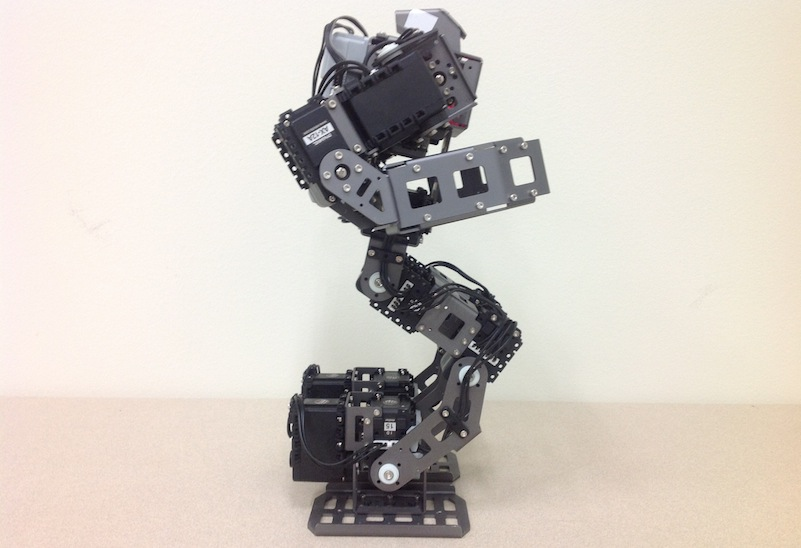
\includegraphics[width=0.3\textwidth]{images/hardware.jpg}
  %% \begin{tabular}{c c}
  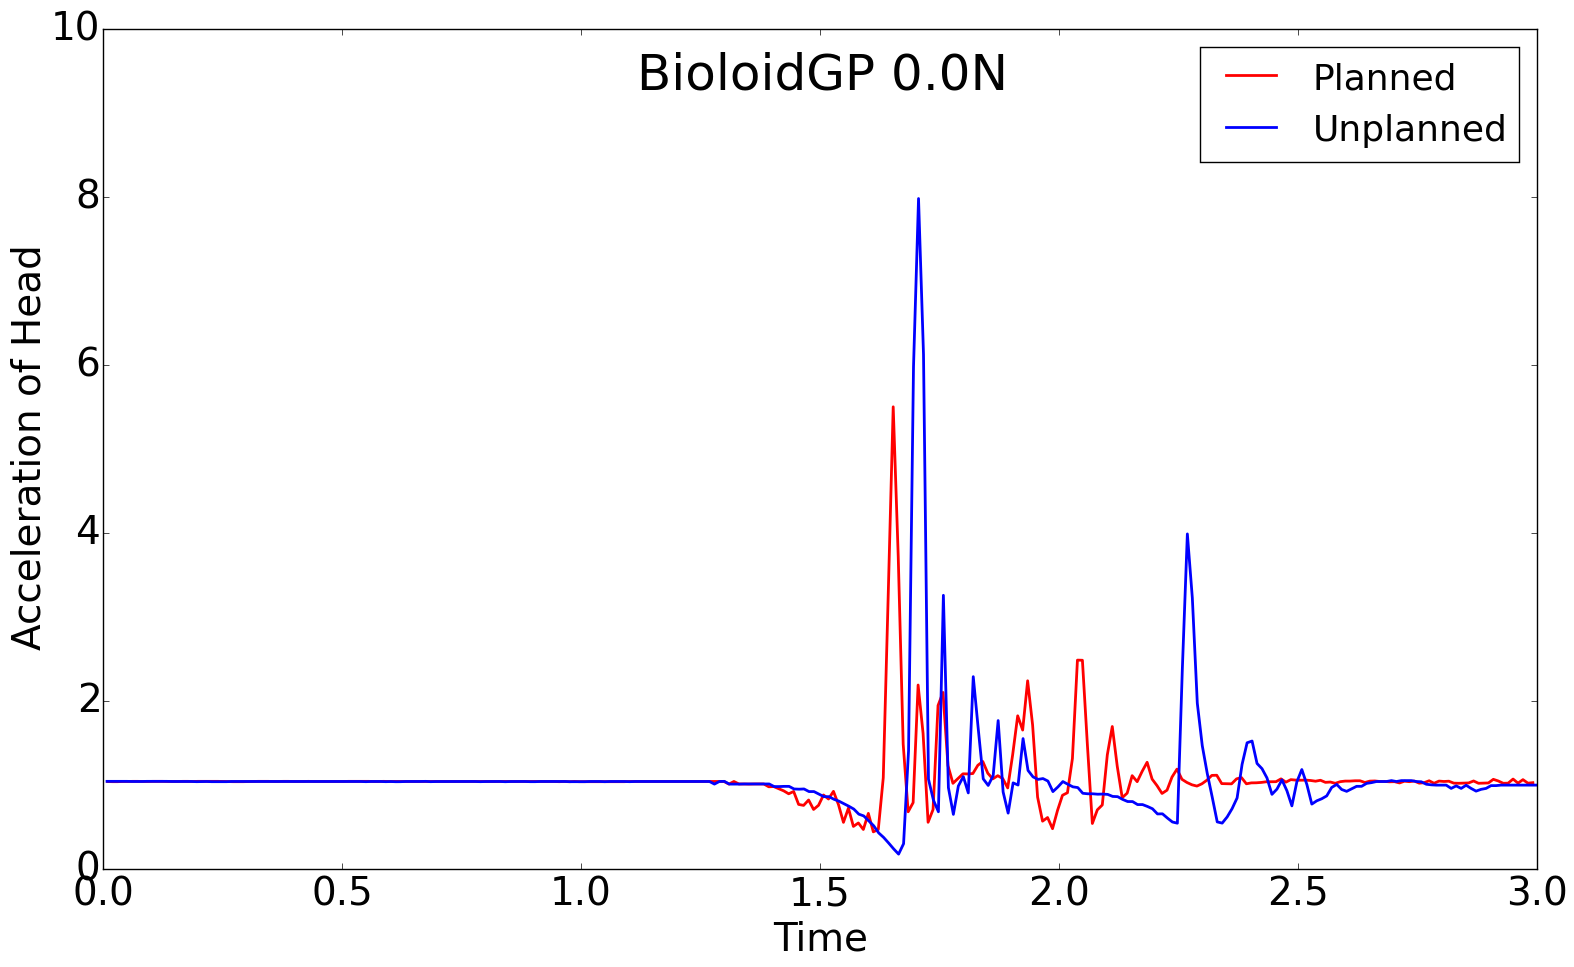
\includegraphics[width=0.34\textwidth]{images/accel00.png}
  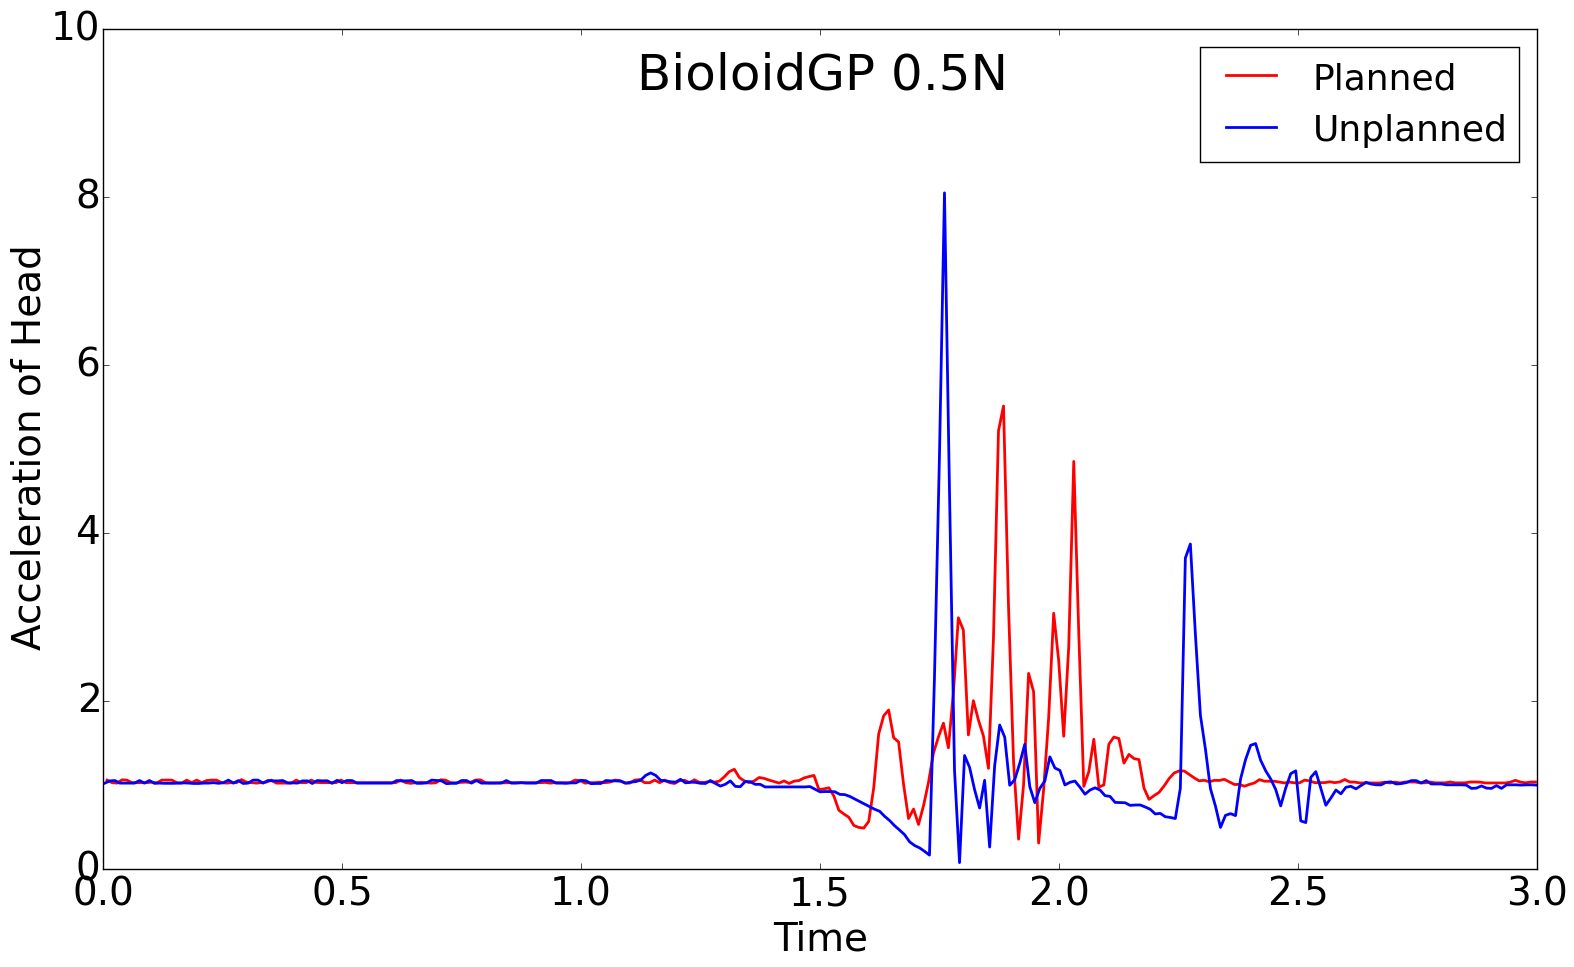
\includegraphics[width=0.34\textwidth]{images/accel01.png}
  %% \end{tabular}
  \caption{We measured the acceleration at the head of BioloidGP (Left). 
    For both $0.0$N (Middle) and $0.5$N (Right) cases, the planned motions
      (Red) yielded about 68\% of the maximum acceleration of the unplanned
      motions (Blue).}
  \label{fig:falling_hardware}
\end{figure}

Finally, we ran two experiments on the hardware of BioloidGP
(\figref{falling_hardware}). In the first experiment, BioloidGP started with
a statically unbalanced position and zero velocity. The optimal plan
simply used hands to stop the COM from descending. In the second
experiment, the robot was pushed forward by a
linear actuator with the magnitude of $0.5$N. In this case,
BioloidGP used two contacts, knees and hands, to stop the fall. We
attached an accelerometer to the head of BioloidGP and measured the
maximum acceleration during the fall. For both cases, the maximum
acceleration resulted from our algorithm was about
68\% of that resulted from the unplanned motion (\figref{falling_hardware}).

We ran an additional experiment to show that BioloidGP is capable of
deploying the rolling strategy to stop a high-speed fall. We gave
BioloidGP a strong shove by hand at the beginning. The large initial
momentum resulted in a somersault motion with five contacts. Due to
the safety concern, we did not perform the same experiment to produce
an unplanned motion for comparison. All the hardware experiments can
be viewed in the supplementary video.


% the robot loses its balance due to the gravity without
%   perturbation. 
%   In the second, the robot is pushed forward by 0.5N perturbation given by a
%   linear actuator.  
%   Due to the absence of contact sensors, the target pose is advanced by timing.
%   Instead of measuring impulses, we measure damage as the acceleration at the
%   head of the robot and compare the peak.

% \updated{When it looses balance, BioloidGP made a contact at hands that tries
%   to stop with the highest final COM position.
%   For 0.5N push, BioloidGP takes two steps, knees and hands.
%   For both cases, the maximum acceleration of the controlled motion is around
%   68\% of the uncontrolled motion (\figref{falling_hardware}).}


%%%%%%%%%%%%%%%%%%%%%%%%%%%%%%%%%%%%%%%%%%%%%%%%%%%%%%%%%%%%%%%%%%%%%%%%%%%%%%%%
\subsection{Limitations}
Our algorithm has a few limitations. First, the planning takes $1.0$
to $10.0$ seconds to compute in all our experiments. As a result, the
algorithm is not ready to deploy in the real-world situations where
robots need to react autonomously in real-time. However, our
preliminary results show that an optimized contact plan typically can
reduce damage for a range of initial conditions, not just for the
initial conditions it was optimized for. For example, the optimized
contact plan of BioloidGP for $5.0$N push yields 35\% to 50\% of the
maximum impulse for pushes ranging from $2.5N$ to $6.5$N.  The
preliminary results imply that it is possible to precompute a set of
contact plans which sparsely covers the space of all possible initial
conditions. The robot can choose one plan with the most similar
initial condition to the online situation to execute.

The two criteria we use to exclude the infeasible stoppers in
\algref{falling_stopper} are tend to be too conservative. In particular, using
$\hat{\theta}_2(c_1, c_2)$ from the initial robot configuration to
approximate the position of the stopper at each impact moment can be
erroneous as the angles between limbs are continuously changing during
the fall. Adding other criteria, such as torque limits, to exclude
infeasible stoppers might lead to more efficient search.

% In our approach, the feasibility test of stoppers in \algref{falling_stopper}
%   is an important component for generating a valid abstract plan $\mathcal{P}$.
%   Although we used two criteria, they are not accurate enough to reject all bad
%   stoppers.  
%   For instance, our definition of the initial angle $\theta_2^0(c_1, c_2)$ is
%   does not consider the changes of angles in the previous contacts, which makes
%   the test inaccurate.
  %% Indeed, modeling a tight bound in the space of the abstract model is 
  %% a difficult problem.
  %% For instance, the same configurations of the pendulum and the stopper can
  %% be achieved by very different full-body poses.
  % The practical approach is to superimpose more constraints based on the
  % specification of the robot, such as torque limits or mass distributions.

Our algorithm is limited to planar motion. Falls that require
non-planar plans, such as those described in \cite{Yun:2014:TFC} and
\cite{Goswami:2014:DCF} cannot be effectively stopped by our
algorithm. One possible future work is to use a more complex model,
such as a reaction mass pendulum with a rigid body inertial mass,
proposed by \cite{Goswami:2014:DCF}.

Finally, we observed that many motions did not end with an balanced,
erect stance, because a balanced final pose is not the goal of our
planning algorithm. If a balanced final pose is a desired feature, we
can simply activate an additional static balance controller after the last contact
is executed. Because the momentum at the final contact is near zero,
maintaining a static balance is not a difficult task.
% \sehoon{In fact, I did the exactly same thing for 0.5N of GP, running a balance
%   controller after stepping. Would it be worth to explicitly mention?}

% Another limitation comes from our planarity assumption on the falling
%   motion.
%   Therefore, our problem cannot illustrate non-planar falls such as
%   a self-orienting fall \cite{Yun:2014:TFC} or a direction changing fall
%   \cite{Goswami:2014:DCF}.
%   One possible extension is to use a more complex model, such as a
%   reaction mass pendulum that the pendulum has a rigid body inertial mass,
%   proposed in \cite{Goswami:2014:DCF}.
